
\documentclass[
	11pt,
]{beamer}

% Specifies where to look for included images (trailing slash required)

\usepackage{booktabs} % Allows the use of \toprule, \midrule and \bottomrule for better rules in tables

%----------------------------------------------------------------------------------------
%	SELECT LAYOUT THEME
%----------------------------------------------------------------------------------------

% Beamer comes with a number of default layout themes which change the colors and layouts of slides. Below is a list of all themes available, uncomment each in turn to see what they look like.

%\usetheme{default}
%\usetheme{AnnArbor}
%\usetheme{Antibes}
%\usetheme{Bergen}
%\usetheme{Berkeley}
%\usetheme{Berlin}
%\usetheme{Boadilla}
%\usetheme{CambridgeUS}
%\usetheme{Copenhagen}
%\usetheme{Darmstadt}
%\usetheme{Dresden}
%\usetheme{Frankfurt}
%\usetheme{Goettingen}
%\usetheme{Hannover}
%\usetheme{Ilmenau}
%\usetheme{JuanLesPins}
%\usetheme{Luebeck}
\usetheme{Madrid}
%\usetheme{Malmoe}
%\usetheme{Marburg}
%\usetheme{Montpellier}
%\usetheme{PaloAlto}
%\usetheme{Pittsburgh}
%\usetheme{Rochester}
%\usetheme{Singapore}
%\usetheme{Szeged}
%\usetheme{Warsaw}

%----------------------------------------------------------------------------------------
%	SELECT COLOR THEME
%----------------------------------------------------------------------------------------

% Beamer comes with a number of color themes that can be applied to any layout theme to change its colors. Uncomment each of these in turn to see how they change the colors of your selected layout theme.

%\usecolortheme{albatross}
%\usecolortheme{beaver}
%\usecolortheme{beetle}
%\usecolortheme{crane}
%\usecolortheme{dolphin}
%\usecolortheme{dove}
%\usecolortheme{fly}
%\usecolortheme{lily}
%\usecolortheme{monarca}
%\usecolortheme{seagull}
%\usecolortheme{seahorse}
%\usecolortheme{spruce}
%\usecolortheme{whale}
%\usecolortheme{wolverine}

%----------------------------------------------------------------------------------------
%	SELECT FONT THEME & FONTS
%----------------------------------------------------------------------------------------

% Beamer comes with several font themes to easily change the fonts used in various parts of the presentation. Review the comments beside each one to decide if you would like to use it. Note that additional options can be specified for several of these font themes, consult the beamer documentation for more information.

 % Typeset using the default sans serif font
\usefonttheme{professionalfonts}
%\usefonttheme{serif} % Typeset using the default serif font (make sure a sans font isn't being set as the default font if you use this option!)
%\usefonttheme{structurebold} % Typeset important structure text (titles, headlines, footlines, sidebar, etc) in bold
%\usefonttheme{structureitalicserif} % Typeset important structure text (titles, headlines, footlines, sidebar, etc) in italic serif
%\usefonttheme{structuresmallcapsserif} % Typeset important structure text (titles, headlines, footlines, sidebar, etc) in small caps serif

%------------------------------------------------

%\usepackage{mathptmx} % Use the Times font for serif text
%\usepackage{palatino} % Use the Palatino font for serif text
\usepackage[utf8]{inputenc} % allow utf-8 input
\usepackage[T1]{fontenc}    % use 8-bit T1 fonts
\usepackage{hyperref}       % hyperlinks
\usepackage{url}            % simple URL typesetting
\usepackage{booktabs}       % professional-quality tables
\usepackage{amsfonts}       % blackboard math symbols
\usepackage{nicefrac}       % compact symbols for 1/2, etc.
\usepackage{microtype}      % microtypography
\usepackage{lipsum}
\usepackage{fancyhdr}       % header
\usepackage{graphicx}       % graphics
\usepackage{physics}
\usepackage{xcolor}
\usepackage{amsmath}
\usepackage{algorithm}
\usepackage{algpseudocode}
%\usepackage{helvet} % Use the Helvetica font for sans serif text
 % Use the Open Sans font for sans serif text
%\usepackage[default]{FiraSans} % Use the Fira Sans font for sans serif text
%\usepackage[default]{lato} % Use the Lato font for sans serif text

%----------------------------------------------------------------------------------------
%	SELECT INNER THEME
%----------------------------------------------------------------------------------------

% Inner themes change the styling of internal slide elements, for example: bullet points, blocks, bibliography entries, title pages, theorems, etc. Uncomment each theme in turn to see what changes it makes to your presentation.

%\useinnertheme{default}
\useinnertheme{circles}
%\useinnertheme{rectangles}
%\useinnertheme{rounded}
%\useinnertheme{inmargin}

%----------------------------------------------------------------------------------------
%	SELECT OUTER THEME
%----------------------------------------------------------------------------------------

% Outer themes change the overall layout of slides, such as: header and footer lines, sidebars and slide titles. Uncomment each theme in turn to see what changes it makes to your presentation.

%\useoutertheme{default}
%\useoutertheme{infolines}
%\useoutertheme{miniframes}
%\useoutertheme{smoothbars}
%\useoutertheme{sidebar}
%\useoutertheme{split}
%\useoutertheme{shadow}
%\useoutertheme{tree}
%\useoutertheme{smoothtree}

%\setbeamertemplate{footline} % Uncomment this line to remove the footer line in all slides
%\setbeamertemplate{footline}[page number] % Uncomment this line to replace the footer line in all slides with a simple slide count

%\setbeamertemplate{navigation symbols}{} % Uncomment this line to remove the navigation symbols from the bottom of all slides

%----------------------------------------------------------------------------------------
%	PRESENTATION INFORMATION
%----------------------------------------------------------------------------------------
\setbeamertemplate{itemize item}[ball]
\setbeamertemplate{enumerate item}[ball]
\title[CS115 - Math for Computer Science]{Recurrent Neural Networks (RNNs) \\ and the Exploding \& Vanishing Gradient Problems} % The short title in the optional parameter appears at the bottom of every slide, the full title in the main parameter is only on the title page

% \subtitle{and the Exploding and Vanishing Gradient Problems} % Presentation subtitle, remove this command if a subtitle isn't required

\author[Nhom 10]{
                    Le Gia Khang \and 21522189 \\
                    Bui Manh Hung \and 21522110 \\
                    Nguyen Hoang Tan \and 21521413 \\
                    Pham Tram Anh \and 21520587 \\
                    Le Thi Kim Yen \and 21521695 \\} % Presenter name(s), the optional parameter can containa shortened version to appear on the bottom of every slide, while the main parameter will appear on the title slide

\institute[UIT]{\fontsize{10}{12}\selectfont \textbf{University of Information Technology} \\ \smallskip \textit{}} % Your institution, the optional parameter can be used for the institution shorthand and will appear on the bottom of every slide after author names, while the required parameter is used on the title slide and can include your email address or additional information on separate lines

\date[\today]{ \\ \today} % Presentation date or conference/meeting name, the optional parameter can contain a shortened version to appear on the bottom of every slide, while the required parameter value is output to the title slide

%----------------------------------------------------------------------------------------

\begin{document}

%----------------------------------------------------------------------------------------
%	TITLE SLIDE
%----------------------------------------------------------------------------------------
\setcounter{tocdepth}{1}
\begin{frame}
	\titlepage % Output the title slide, automatically created using the text entered in the PRESENTATION INFORMATION block above
\end{frame}

%----------------------------------------------------------------------------------------
%	TABLE OF CONTENTS SLIDE
%----------------------------------------------------------------------------------------

% The table of contents outputs the sections and subsections that appear in your presentation, specified with the standard \section and \subsection commands. You may either display all sections and subsections on one slide with \tableofcontents, or display each section at a time on subsequent slides with \tableofcontents[pausesections]. The latter is useful if you want to step through each section and mention what you will discuss.

\begin{frame}
	\frametitle{References}
	The contents of this document are taken mainly from the follow sources:
	\begin{itemize}
		\item Robin M.Schmidt, Recurrent Neural Networks (RNNs): a gentle introductionand overview\footnote[1]{\url{https://arxiv.org/pdf/1912.05911.pdf}};
		\item Razvan Pascanu, Tomas Mikolov, Yoshua Bengio, On the difficulty of training RNNs\footnote[2]{\url{https://arxiv.org/pdf/1211.5063.pdf}}
		\item Yoshua Bengio, Patrice Simard, Paolo Frasconi, Learning long-term dependencies with gradients descent is difficult\footnote[3]{\url{https://www.researchgate.net/profile/Y-Bengio/publication/5583935_Learning_long-term_dependencies_with_gradient_descent_is_difficult/links/546b702d0cf2397f7831c03d/Learning-long-term-dependencies-with-gradient-descent-is-difficult.pdf}}
	\end{itemize}

	%\footnote[2]{https://arxiv.org/pdf/1211.5063.pdf}
	%\footnote[3]{https://www.researchgate.net/profile/Y-Bengio/publication/5583935_Learning_long-term_dependencies_with_gradient_descent_is_difficult/links/546b702d0cf2397f7831c03d/Learning-long-term-dependencies-with-gradient-descent-is-difficult.pdf}
\end{frame}
\begin{frame}
	\frametitle{Table of Contents} % Slide title, remove this command for no title
	
	\tableofcontents % Output the table of contents (all sections on one slide)
	%\tableofcontents[pausesections] % Output the table of contents (break sections up across separate slides)
\end{frame}

%----------------------------------------------------------------------------------------
%	PRESENTATION BODY SLIDES
%----------------------------------------------------------------------------------------

\section{Introduction \& Notation} % Sections are added in order to organize your presentation into discrete blocks, all sections and subsections are automatically output to the table of contents as an overview of the talk but NOT output in the presentation as separate slides
\begin{frame}
	\frametitle{Table of Contents}

	\tableofcontents[currentsection]
\end{frame}
%------------------------------------------------
\subsection{Sequential Data}
\begin{frame}
	\frametitle{Sequential Data}
	\begin{itemize}
		\item Sequential Data refers to any data that contain elements that are ordered into sequences. 
	\bigskip
		\item Examples include time series, DNA sequences (see biomedical informatics) and sequences of user actions.
	\bigskip
	\begin{block}{Question ?}
		\fontsize{10}{12}\selectfont \textbf{Named-entity Recognition for person names:} \\
		\smallskip
		\;\;\;\;\;\;\;\;\;\;\;\;\;\;\;\;\;\;\;\textcolor{blue}{Harry Potter} and \textcolor{blue}{Hermione Granger} invented a new spell.
	\end{block}
	\bigskip
		\item Machine learning models that input or output data sequences are known as sequence models.
\end{itemize}
\end{frame}
\begin{frame}
	\frametitle{What's Recurrent Neural Networks (RNNs)}
	\begin{itemize}
		\item Recurrent Neural Networks (RNNs) are a type of neural network architecture which is mainly used to detect patterns
		in a sequence of data.
		\bigskip
		\item However, they are also applicable to images if these get
		respectively decomposed into a series of patches and treated as a sequence.
		\bigskip
		\item What differentiates Recurrent Neural Networks from Feedforward Neural Networks also known as Multi-Layer Perceptrons
		(MLPs) is how information gets passed through the network.
	\end{itemize}
\end{frame}
\subsection{Model Architecture}
\begin{frame}
	\frametitle{Model Architecture}
	\begin{itemize}
		\item The RNN has cycles and transmits information back into itself. This enables them to extend
	the functionality of Feedforward Networks to also take into account previous inputs $X_{0:t-1}$ and not only the current
	input $X_t$.
	\end{itemize}
	\begin{figure}
		\centering
		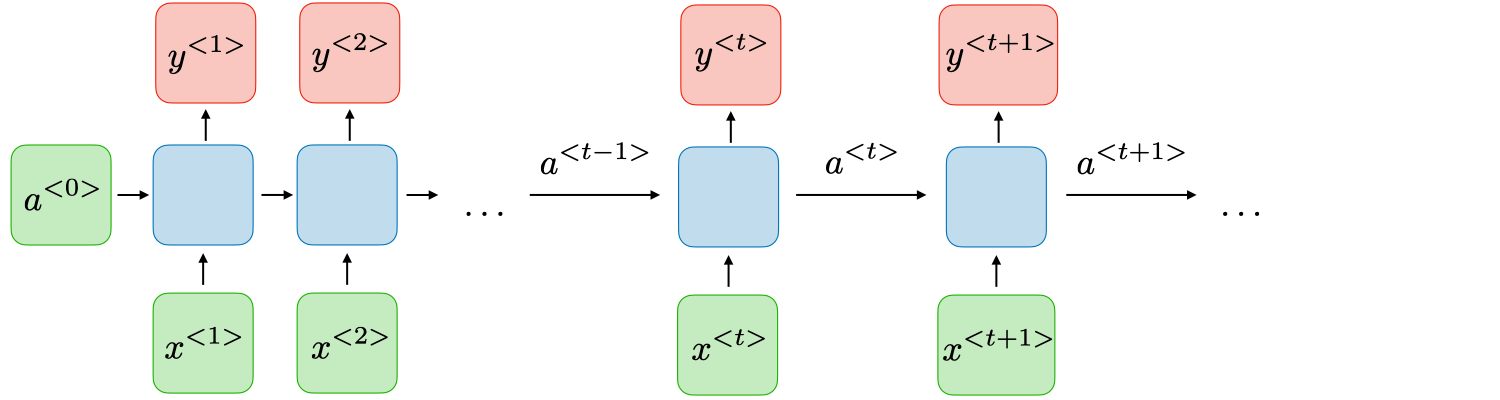
\includegraphics[scale=0.25]{Images/architecture-rnn-ltr.png}
	\end{figure}
\end{frame}
\begin{frame}
	\frametitle{Model Architecture}
	\begin{itemize}
		\item We denote the hidden state and the input at time step t respecively as $\mathbf{H}_t$ and $X_t$
Further, we use $\mathbf{W}_{xh}$, $\mathbf{W}_{hh}$, $\mathbf{W}_{ho}$ and a bias $b_h$ as shared parameters. Lastly, all these informations get passed to a activation function $\phi$ which is usually a logistic sigmoid or
tanh function.
	\end{itemize}
	\begin{block}{Hidden state at the time step t}
		\begin{equation*}
			\mathbf{H}_t = \phi_h(\mathbf{X}_t\,\mathbf{W}_{xh} + \mathbf{H}_{t-1}\,\mathbf{W}_{hh} + \mathbf{b}_h)
		\end{equation*}
	\end{block}
	\smallskip
	\begin{block}{Output at time step t}
		\begin{equation*}
			\mathbf{O}_t = \phi_o (\mathbf{H}_t\,\mathbf{W}_{ho} + \mathbf{b}_o)
		\end{equation*}
	\end{block}
\end{frame}


\subsection{Loss Function}

\begin{frame}
	\frametitle{Loss Function}
	\begin{itemize}
		\item Loss function evaluates performance of the network by comparing the output $\mathbf{y}_t$ with the corresponding target $\mathbf{z}_t$
		defined as:
		\bigskip
	\begin{block}{Loss Function}
		\begin{equation*}
			L(\mathbf{y,z}) = \sum_{t=1}^T L_t(\mathbf{y_t, z_t})
		\end{equation*}
	\end{block}
		\bigskip
		\item Selection of the loss function is problem dependent. Some
	popular loss function are Euclidean distance and Hamming distance and cross-entropy.
\end{itemize}
\end{frame}

\begin{frame}
	\frametitle{Pros and Cons}
	\large{\textcolor{blue}{\textbf{Benefits}}}
	\begin{itemize}
		\item Possibility of processing input of any length;
		\item Model size not increasing with size of input;
		\item Computation takes into account historical information;
		\item Weights are shared across time
	\end{itemize}
	\bigskip
	\large{\textcolor{red}{\textbf{Costs}}}
	\begin{itemize}
		\item Computation being slow;
		\item Difficulty of accessing information from a long time ago;
		\item Cannot consider any future input for the current state;
	\end{itemize}
\end{frame}

\begin{frame}
	\frametitle{Various usage of RNN}
	\large{\textcolor{blue}{\textbf{One to One RNN}}}
	\begin{itemize}
		\item This type of neural network is known as the Vanilla Neural Network. It's used for general machine learning problems, which has a single input and a single output.
	\end{itemize}
	\begin{figure}[h]
		\centering
		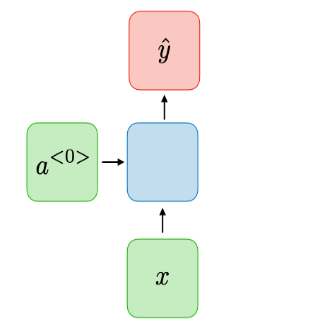
\includegraphics[scale=0.5]{Images/one_to_one.png}
		\caption{Vanilla Neural Network}
	\end{figure}
\end{frame}

%------------------------------------------------
\begin{frame}
	\frametitle{Various usage of RNN}
	\large{\textcolor{blue}{\textbf{One to Many RNN}}}
	\begin{itemize}
		\item A type of RNN that gives multiple outputs when given a single input. It takes a fixed input size and gives a sequence of data outputs.
		\item Its applications can be found in Music Generation and Image Captioning.
	\end{itemize}
	\begin{figure}[h]
		\centering
		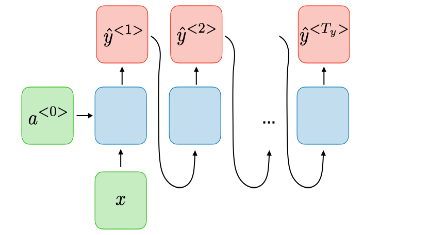
\includegraphics[scale=0.5]{Images/one_to_many.png}
		\caption{One-to-Many mode}
	\end{figure}
\end{frame}

\begin{frame}
	\frametitle{Various usage of RNN}
	\large{\textcolor{blue}{\textbf{Many to One RNN}}}
	\begin{itemize}
		\item Many-to-One is used when a single output is required from multiple input units or a sequence of them. It takes a sequence of inputs to display a fixed output.
		\item Sentiment Analysis is a common example of this type of Recurrent Neural Network.
	\end{itemize}
	\begin{figure}[h]
		\centering
		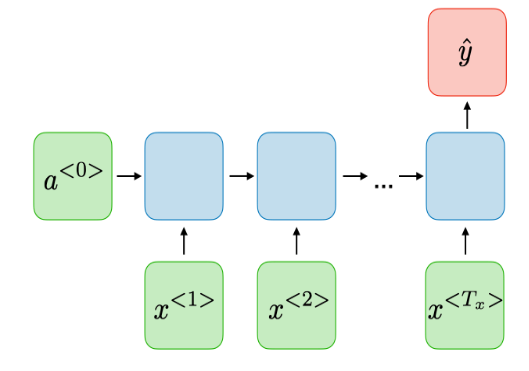
\includegraphics[scale=0.4]{Images/many_to_one.png}
		\caption{Many to One mode}
	\end{figure}
\end{frame}

\begin{frame}
	\frametitle{Various usage of RNN}
	\large{\textcolor{blue}{\textbf{Many to Many RNN}}}
	\begin{itemize}
		\item Many-to-Many is used to generate a sequence of output data from a sequence of input units.
		\item This type of RNN is further divided into the following two subcategories:
		\begin{enumerate}
			\item \textcolor{green}{Equal Unit Size:} In this case, the number of both the input and output units is the same. A common application can be found in Name-Entity Recognition.
			\item \textcolor{green}{Unequal Unit Size} In this case, inputs and outputs have different numbers of units. Its application can be found in Machine Translation.
		\end{enumerate}
	\end{itemize}
	\par
	\raisebox{-.5\height}{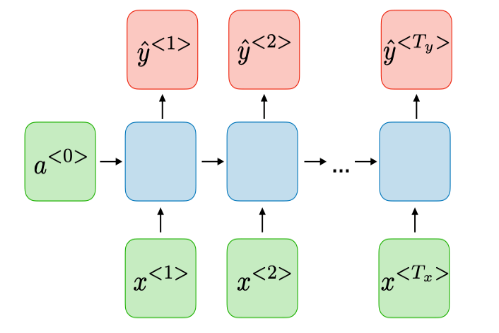
\includegraphics[scale=0.3]{Images/many_to_many1.png}}%
	\hfill
	\raisebox{-.5\height}{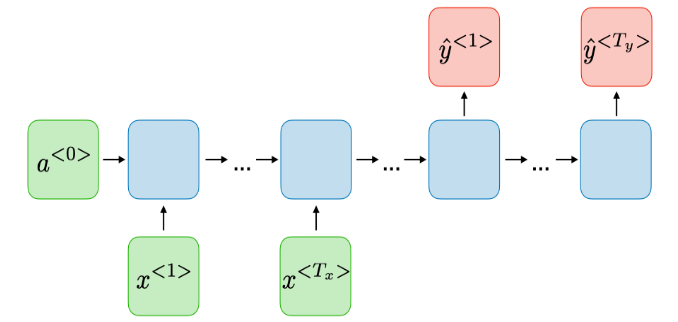
\includegraphics[scale=0.3]{Images/many_to_many2.png}}%
	\par
\end{frame}

\section{Training Recurrent Neural Networks}
\begin{frame}
	\frametitle{Table of Contents}
	\tableofcontents[currentsection]
\end{frame}
%------------------------------------------------

\subsection{Initializations}

\begin{frame}
	\frametitle{Initializations}

	\begin{itemize}
		\item A general rule is to assign small values to the weights. A
		Gaussian draw with a standard deviation of $0.001$ or $0.01$ is a reasonable choice.
		\bigskip
		\item The biases are usually set to zero,
		but the output bias can also be set to a very small value.
		\bigskip
		\item However, the initialization of parameters is dependent on the
		task and properties of the input data such as dimensionality. 
	\end{itemize}

\end{frame}

%------------------------------------------------

\subsection{Gradient-based Learning Methods}

\begin{frame}
	\frametitle{Gradient-based Learning Methods}
	\begin{itemize}
		\item Gradient descent (GD) adjusts the
weights of the model by finding the error function derivatives with respect to each member of the weight matrices.
	
 	\bigskip % Vertical whitespace
  
        \begin{block}{Batch Gradient Descent}
		Computing the gradient for the whole dataset in each optimization iteration to perform a single update as
		\begin{equation*}
            \theta_{t+1} = \theta_t - \frac{\lambda}{U}\sum_{k=1}^U \pdv{\ell_k}{\theta}
		\end{equation*}
	\end{block}
	
 	\bigskip % Vertical whitespace

	 \item However, computing error-derivatives through time is difficult. This is mostly due to the
	 relationship among the parameters and the dynamics of the RNN, that is highly unstable and makes GD ineffective.
	\end{itemize}
\end{frame}

%------------------------------------------------

\begin{frame}
	\frametitle{Gradient-based Learning Methods}
	\begin{itemize}
		\item Gradient-based algorithms have difficuly in capturing dependencies as the duratiton of dependencies increases.
		\bigskip
		\item The derivatives of the loss function with respect to the weights only consider the current state, without using the history information for weights updating.
		\bigskip
		\item  RNNs cannot learn long-range temporal dependencies when GD is used for training.
	\end{itemize}
\end{frame}

\subsection{Back-propagation through time (BPTT)}

\begin{frame}
	\frametitle{Back-propagation through time (BPTT)}
	\begin{itemize}
		\item Backpropagation Through Time (BPTT) is the adaption of the backpropagation algorithm for RNNs.
		\bigskip 
		\item BPTT unfolds the RNN to construct a traditional Feedfoward Neural Network where we can apply backpropagation.
        \bigskip % Vertical whitespace
		\par
		\raisebox{-.5\height}{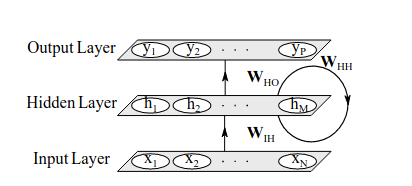
\includegraphics[scale=0.4]{Images/folded_rnn.png}}%
		\hfill
		\raisebox{-.5\height}{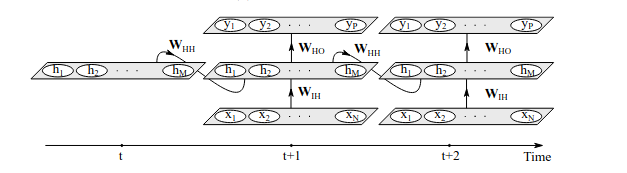
\includegraphics[scale=0.4]{Images/unfolded_rnn.png}}%
		\par

			
\end{itemize}
\end{frame}

%------------------------------------------------

\begin{frame}
	\frametitle{Back-propagation through time (BPTT)}

		Since we have three weight matrices $\mathbf{W}_{xh}, \mathbf{W}_{hh}$ and $\mathbf{W}_{ho}$ we need to
compute the partial derivative to each of these weight matrices using the
chain rule.
		\smallskip
        \begin{block}{Partial derivative with respect to $\mathbf{W}_{ho}$}
        \begin{equation*}
            \frac{\partial L}{\partial \mathbf{W}_{ho}} = \sum_{t=1}^{T}\frac{\partial l_t}{\partial \mathbf{O}_t}.\frac{\partial \mathbf{O}_t}{\partial \phi_o}.\frac{\partial \phi_o}{\partial \mathbf{W}_{ho}} = \sum_{t=1}^{T}\frac{\partial l_t}{\partial \mathbf{O}_t}.\frac{\partial \mathbf{O}_t}{\partial \phi_o}.\mathbf{H}_t
        \end{equation*}
		\end{block}
	\begin{block}{Partial derivative with respect to $\mathbf{W}_{hh}$}
        \begin{equation*}
			\begin{split}
            \pdv{L}{\mathbf{W}_{hh}} &= \sum_{t=1}^T \pdv{\ell_t}{\mathbf{O}_t} \cdot \pdv{\mathbf{O}_t}{\phi_o} \cdot \pdv{\phi_o}{\mathbf{H}_t} \cdot \pdv{\mathbf{H}_t}{\phi_h} \cdot \pdv{\phi_h}{\mathbf{W}_{hh}} \\
									 &= \sum_{t=1}^T \pdv{\ell_t}{\mathbf{O}_t} \cdot \pdv{\mathbf{O}_t}{\phi_o} \cdot \mathbf{W}_{ho} \cdot \pdv{\mathbf{H}_t}{\phi_h} \cdot \pdv{\phi_h}{\mathbf{W}_{hh}} 
			\end{split}
        \end{equation*}
	\end{block}

\end{frame}

\begin{frame}
	\frametitle{Back-propagation through time (BPTT)}
	\begin{itemize}
		\item Since each $\mathbf{H}_t$ depends on the previous time step we can substitute the last part from above equation
	\begin{block}{Partial derivative with respect to $\mathbf{W}_{hh}$}
		\begin{equation*}
			\pdv{L}{\mathbf{W}_{hh}} = \sum_{t=1}^T \pdv{\ell_t}{\mathbf{O}_t} \cdot \pdv{\mathbf{O}_t}{\phi_o} \cdot \mathbf{W}_{ho} \sum_{k=1}^t \pdv{\mathbf{H}_t}{\mathbf{H}_k} \cdot \pdv{\mathbf{H}_k}{\mathbf{W}_{hh}}
		\end{equation*}
	\end{block}
		\item Similarly, we have the partial derivative with respect to $\mathbf{W}_{xh}$ as below
	\begin{block}{Partial derivative with respect to $\mathbf{W}_{xh}$}
		\begin{equation*}
			\pdv{L}{\mathbf{W}_{xh}} = \sum_{t=1}^T \pdv{\ell_t}{\mathbf{O}_t} \cdot \pdv{\mathbf{O}_t}{\phi_o} \cdot \mathbf{W}_{ho} \sum_{k=1}^t \pdv{\mathbf{H}_t}{\mathbf{H}_k} \cdot \pdv{\mathbf{H}_k}{\mathbf{W}_{xh}}
		\end{equation*}
	\end{block}
\end{itemize}
\end{frame}

\begin{frame}
	\frametitle{Back-propagation through time (BPTT)}
	\begin{itemize}
		\item In order to transport the error through time from timestep t back
		to timestep k we can have
	\begin{block}{}
		\begin{equation*}
			\pdv{\mathbf{H}_t}{\mathbf{H}_k} = \prod_{i = k + 1}^t \pdv{\mathbf{H}_i}{\mathbf{H}_{i-1}}
		\end{equation*}
	\end{block}
		\item We can consider previous equation as a Jacobian matrix for the hidden state parameter as
	\begin{block}{}
		\begin{equation*}
			\prod_{i = k + 1}^t \pdv{\mathbf{H}_i}{\mathbf{H}_{i-1}} = \prod_{i = k+1}^t \mathbf{W}_{hh}^T diag(\phi'_{h}(\mathbf{H}_{i-1}))
		\end{equation*}
	\end{block}
\end{itemize}
\end{frame}


\section{Exploding and Vanishing Gradient}
\begin{frame}
	\frametitle{Table of Contents}
	\tableofcontents[currentsection]
\end{frame}

\begin{frame}
	\frametitle{Vanishing Gradient}
	\begin{itemize}
		\item This problem refers to the exponential shrinking of gradient
		magnitudes as they are propagated back through time.
		\bigskip
		\item This phenomena causes memory of the network to ignore long
		term dependencies and hardly learn the correlation between
		temporally distant events
		\bigskip
		\item There are two reasons for that:
		\begin{enumerate}
			\item Standard nonlinear functions have a gradient which is almost everywhere close to zero;
			\item The magnitude of gradient is multiplied over and over by the recurrent matrix as it is back-propagated through time.
		\end{enumerate}
	\end{itemize}
\end{frame}

\begin{frame}
	\frametitle{Vanishing Gradient}
	\begin{itemize}
		\item It is possible to use spectral radius to generalize it to the non-linear function $\phi'_h$ by bounding it with $\gamma \in R$
		such as
		\bigskip
	\begin{block}{}
		\begin{equation*}
			\norm{diag(\phi'_h(\mathbf{H}_k))} \; \le \; \gamma
		\end{equation*}
	\end{block}
		\bigskip
		\item The Jacobian matrix $\pdv{\mathbf{H}_{k+1}}{\mathbf{H}_k}$ and the bound
		in previous equation, we can have
	\begin{block}{}
		\bigskip
		\begin{equation*}
			\forall k, \norm{\pdv{\mathbf{H}_{k+1}}{\mathbf{H}_k}}  \le \norm{\mathbf{W}_{hh}^T} \;
			 \norm{diag(\sigma'(\mathbf{H}_k))} <  1
		\end{equation*}
	\end{block}
\end{itemize}
\end{frame}

\begin{frame}
	\frametitle{Vanishing Gradient}
	\begin{itemize}
		\item We can consider $\norm{\pdv{\mathbf{H}_{k+1}}{\mathbf{H}_k}} \le \eta < 1$ such as $\eta \in R$ for each
		step $k$. By continuing it over different timesteps and adding
		the loss function component we can have
		\bigskip
	\begin{block}{}
		\begin{equation*}
			\norm{\pdv{\ell_t}{\mathbf{H}_t} \; (\prod_{i=k}^{t-1} \pdv{\mathbf{H}_{i+1}}{\mathbf{H}_i})} \le \eta^{t-k}  \norm{\pdv{\ell_t}{\mathbf{H}_t}}
		\end{equation*}
	\end{block}
		\bigskip
		\item Finally, we can see that the sufficient condition for
		the gradient vanishing problem to appear is that the largest
		singular value of the recurrent weights matrix $\mathbf{W}_{hh}$
		satisfies $\lambda_1 < \frac{1}{\gamma}$
\end{itemize}
\end{frame}

\begin{frame}
	\frametitle{Exploding Gradient}
	\begin{itemize}
		\item Gradients in training RNNs on long sequences
		may explode as the weights become larger and the norm of
		the gradient during training largely increases.
		\bigskip
		\item  As it is stated before, the necessary condition for this situation to happen is
		$\lambda > \frac{1}{\gamma}$.
	\end{itemize}
\end{frame}

\begin{frame}
	\frametitle{Conclusion for the 2 problems}
	\begin{block}{Vanishing Gradient}
		\begin{equation*}
			 \norm{\pdv{\mathbf{H}_{i+i}}{\mathbf{H}_i}} \;\; < \;\; 1
		\end{equation*}
	\end{block}
	\bigskip
	\bigskip
	\begin{block}{Exploding Gradient}
		\begin{equation*}
			\norm{\pdv{\mathbf{H}_{i+1}}{\mathbf{H}_i}} \;\; > \;\; 1
		\end{equation*}
	\end{block}
\end{frame}

\begin{frame}
	\frametitle{Dealing with the exploding and vanishing gradient}
	\begin{itemize}
		\item To deal with the exploding gradients problem, we propose a solution that involves clipping the norm of the exploded
		gradients when it is too large.
	\begin{figure}[h]
		\centering
		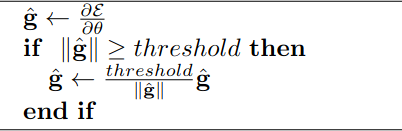
\includegraphics[scale=0.5]{Images/gradient_clipping.png}
	\end{figure}
		\item To deal with the vanishing gradients problem, we propose using LSTMs layers rather than normal Recurrent layers.
	\begin{figure}[h]
		\centering
		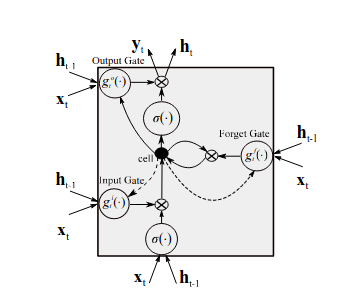
\includegraphics[scale=0.45]{Images/lstm.png}
		\caption{The LSTM memory block with one cell.}
	\end{figure}
\end{itemize}
\end{frame}
%----------------------------------------------------------------------------------------
%	CLOSING SLIDE
%----------------------------------------------------------------------------------------



%----------------------------------------------------------------------------------------

\end{document} 